%% Genetischer Algorithmus.tex
%% $Id: Genetischer Algorithmus.tex 28 2007-01-18 16:31:32Z bless $
%%

Unter dem Begriff der Evalution{\"a}ren Algorithmen (EA) versteht man eine Ansammlung von Techniken und Methoden, die f{\"u}r Optimierungsprobleme eine L{\"o}sung findet, die das Problem n{\"a}herungsweise l{\"o}st. \cite{weicker2015evolutionare} 
%/////Man hat sich bei dem EA an der Biologischen Evolution von Darwin inspirieren lassen. \cite{selzam2003genetische}

%// Die Evalution{\"a}ren Algorithmen sind stochastische Optimierungsverfahren. Mithilfe eines Evolution{\"a}ren Algorithmus (EA) findet man nicht die beste L{\"o}sung f{\"u}r ein Problem, jedoch findet man eine gute L{\"o}sung, die der eigentlichen L{\"o}sung recht nahe kommt.

%% ==============================
\subsection{Evolution in der Biologie}
%% ==============================
Im 19. Jahrhundert hat sich Darwin mit den Gedanken {\"u}ber die Evolution von Lebewesen {\"u}ber mehrere Generationen gemacht. Dabei kam er auf das Prinzip \grqq{Survival of the fittest}. Mit dem Prinzip hat Charles Darwin die Entstehung neuer Arten beschrieben. Dabei haben die Arten {\"u}berlebt, die sich am besten f{\"u}r die Umgebung angepasst haben. Die Arten, die sich an die neue Situation nicht angepasst hatten, sind nach ein paar Generationen zur Minderheit geworden. \cite{hunermann2007brockhaus}

In der Biologie ist jeder lebende Organismus ein \textbf{Individuum}.
Jedes Individuum besitzt Erbinformationen in der Form von Chromosomen. Die Erbinformationen werden auch \textbf{Gene} oder \textbf{DNA} genannt. 
Eine Gruppe von Individuen wird als \textbf{Population} bezeichnet. 

Bei dem EA hat man sich das Verhalten des in der Biologie angeschaut, wie dort die Arten {\"u}ber Generationen hinweg {\"u}berleben und versucht dieses zu adaptieren. \cite{flickevolutionare}

%% ==============================
\subsection{Selektion}
%% ==============================

Eine \textbf{Selektion} ist eine Auswahl von Individuen einer Population. Durch Kombination der Gene der ausgew{\"a}hlten Individuen werden neue Individuen f{\"u}r die n{\"a}chste Generation erzeugt. Diese Kombination wird \textbf{Rekombination} genannt.
Dabei gibt es verschiedene Selektionsstrategien. Man versucht die Individuen zu finden, die eine best m{\"o}glichste L{\"o}sung f{\"u}r ein Problem liefern. \cite{weicker2015evolutionare, flickevolutionare}

%% ==============================
\subsection{Variation}
%% ==============================

F{\"u}r eine Population sollte man zu Beginn eine gro{\ss}e \textbf{Variation} von Individuen mit unterschiedlichen Genen besitzen. 
Anhand eines Beispiels nehme man an, dass man mithilfe einer Evolution eine neue Art von S{\"u}{\ss}igkeiten entwickeln m{\"o}chte. Dabei sollten die Form und Farbe neu bestimmt werden. 
Wenn man jetzt eine Start-Population von Individuen habe, die alle die gleichen Gene besitzen w{\"u}rden, so w{\"u}rde man anhand zwei selektierten Individuen keine {\"A}nderung der n{\"a}chsten Generation erkennen, da die Nachkommen auch alle die gleichen Gene besitzen, falls keine Mutation auftritt.
Damit dieses Verhalten nicht auftritt, versucht man zu Beginn eine gro{\ss}e Variation an Individuen zu erzeugen und diese als Anfangs-Population f{\"u}r einen Evolution{\"a}ren Algorithmus zu nutzen. 
Mittels Rekombination und Mutation wird dabei ein neues Individuum f{\"u}r die n{\"a}chste Generation erzeugt, dass neue Gene bestimmt.
Mithilfe der Rekombination werden verschiedene Gene bei der Fortpflanzung der n{\"a}chsten Generation vermischt und somit neue Gene erzeugt. Die Mutation ist eine Ver{\"a}nderung der Gene eines Individuums, die meistens durch Umwelteinfl{\"u}sse ausgel{\"o}st werden. \cite{flickevolutionare} 

%//Durch Rekombination und Mutation der DNA der Individuen erh{\"a}lt man eine Variation. 
%//Die Rekombination und Mutation erzeugt lediglich ein neues Individuum aus der DNA der zuvor selektierten Individuen.

%//Um die n{\"a}chsten Generationen zu bilden wird eine Rekombination und Mutation auf die DNA der Selektierten Individuen ausgef{\"u}hrt. 
%Die Variation der DNA  spielt eine wichtige Rolle, denn die ist f{\"u}r die nachfolgende Rekombination und Mutation entscheidend f{\"u}r die n{\"a}chsten Generationen. 
%Um bei der Selektion unterschiedliche Individuen ausgew{\"a}hlt werden k{\"o}nnen, ben{\"o}tigt man zun{\"a}chst eine Variation 

%% ==============================
\subsection{Gendrift}
%% ==============================
Unter \textbf{Gendrift} versteht man eine zuf{\"a}llige Ver{\"a}nderung der Genh{\"a}ufigkeit in einer Population, innerhalb einer Evolution. Ein Gendrift tritt bei kleineren Populationen h{\"a}ufiger auf. \cite{brockhausonline} % \cite{gendrift2018brockhaus} 


%% ==============================
\subsection{Allgeimeiner Vorgang eines Evolution{\"a}ren Algorithmus}
%% ==============================
\begin{figure}
	\centering
    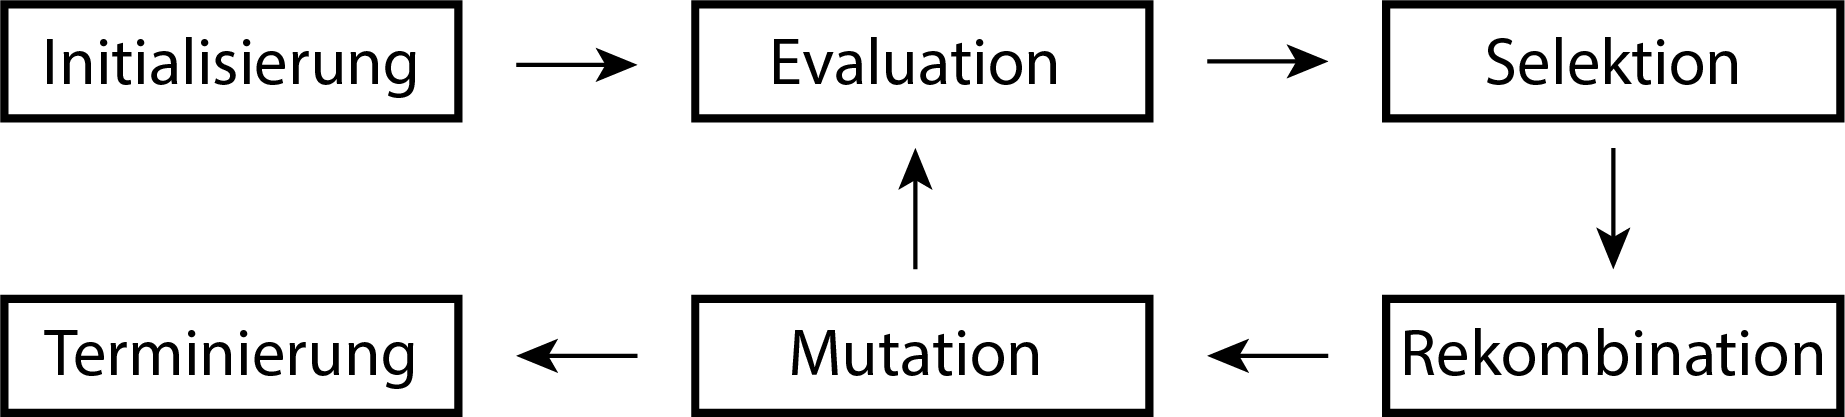
\includegraphics[width=\textwidth]{pics/algoSchritte.png}
    \caption{Ablauf des Algorithmus}
    \label{fig:algoSchritte}
\end{figure}
Der EA besitzt im Allgemeinen immer die gleichen Komponenten. Diese Komponenten werden im folgenden erl{\"a}utert. Dieses Wissen stammt aus den Folgenden Quellen: \cite{shiffman2012nature, flickevolutionare, weicker2015evolutionare}

%% ==============================
\paragraph*{Initialisierung}
%% ==============================
In der Initialisierung erzeugt man sich eine Population von Individuen, die eine zahlreiche Variationen von Genen besitzen. F{\"u}r die Anfangs-Population nimmt man in der Praxis zuf{\"a}llige Individuen oder auch die besten bekanntesten L{\"o}sungskandidaten.

%% ==============================
\paragraph*{Bewertung der Individuen}
%% ==============================
Bevor man eine Evolution f{\"u}r eine Population erzeugen kann, ben{\"o}tigt man Attribute anhand derer man die n{\"a}chste Generation berechnet. Mit einer sogenannten \textbf{Fitnessfunktion} berechnet anhand der Attribute eines Individuums einen \textbf{Fitnesswert}. Der Fitnesswert ist entscheidend f{\"u}r die Selektion.

%Diese Attribute nennt man den \textbf{Fitnesswert}. Der Fitnesswert muss f{\"u}r jedes Individuum der Population bestimmt werden. Der Fitnesswert wird anhand mithilfe einer Fitnessfunktion berechnet. 

%//Bevor man eine neue Population f{\"u}r die n{\"a}chste Generation berechnen kann, muss man zuerst mithilfe einer Fitnessfunktion jedes Induvidiuum einen Fitnesswert bestimmen. 

%% ==============================
\paragraph*{Selektion}
%% ==============================
Die Selektion w{\"a}hlt zwei Individuen als Eltern aus, diese werden anhand des Fitnesswerts der Individuen aus einer Population bestimmt. 
%In der Selektion werden Individuen ausgew{\"a}hlt, die als Paare neue Kinder f{\"u}r die n{\"a}chste Generation bilden.
%Bei der Selektion w{\"a}hlt man Individuen aus der Population.
%Bei der Selektion w{\"a}hlt man die Individuen jeweils Individuen aus einer Population aus. 
Es werden die Individuen bevorzugt, die einen hohen Fitnesswert aufweisen. Diese ermittelten Eltern werden mittels der Rekombination und Mutation weiter verarbeitet.

%% ==============================
\paragraph*{Rekombination}
%% ==============================
Die selektierten Eltern werden in diesem Schritt einen Nachfahren f{\"u}r die n{\"a}chste Generation erzeugen. Dabei werden die jeweiligen Gene der Eltern kombiniert und an die n{\"a}chste Generation vererbt. Die Kombinationsm{\"o}glichkeiten h{\"a}ngen davon ab, wie die Gene repr{\"a}sentiert sind.
Die neuen Individuen werden in die Population f{\"u}r die n{\"a}chste Generation hinzugef{\"u}gt.

%//Die Gene der ausgew{\"a}hlten Eltern werden miteinander kombiniert und bilden die Gene des neuen Induvidiuum f{\"u}r die Population der n{\"a}chsten Generation. Hier gibt es verschiedene Kombinationsm{\"o}glichkeiten, die angewendet werden k{\"o}nnen.

%% ==============================
\paragraph*{Mutation}
%% ==============================
Nach der Rekombination besteht eine Chance, dass die Gene des Nachkommens mutieren k{\"o}nnen. 
%Es besteht eine Chance, dass die Gene der Individuen der neuen Generation sich mutieren k{\"o}nnen. 

%% ==============================
\paragraph*{Terminierung}
%% ==============================

Man f{\"u}hrt f{\"u}r eine Generation die Selektion, Rekombination und Mutation so oft aus, bis man die gleiche Anzahl an Individuen f{\"u}r die n{\"a}chste Generation erzeugt hat.
Der Vorgang der Evaluierung, Selektion, Rekombination und Mutation muss f{\"u}r jede neue Generation durchgef{\"u}hrt werden. 
Die neu erzeugte Population wird als Eingabe f{\"u}r die neue Generation verwendet. 
Dabei wird der Algorithmus so lange ausgef{\"u}hrt, bis eine hinreichende Abbruchbedingung erreicht worden ist. 
Je nach Definition der Terminierung, kann nach einer festen Anzahl an Generationen oder erst nachdem es keine signifikanten {\"A}nderungen der Generationen mehr gibt, der EA terminiert werden.
Das dadurch erzeugte Ergebnis ist eine n{\"a}herungsweise L{\"o}sung f{\"u}r das Problem.

%% ==============================
\subsection{Darstellung}
%% ==============================
Es gibt verschiedene Darstellungsm{\"o}glichkeiten von Genen, die meist verwendeten Darstellungen werden im Folgenden erläutert. Das wissen, wurde aus der Ausarbeitung von \cite{flickevolutionare, shiffman2012nature, DillmannZoeller2017} entnommen.

Eine \textbf{Lineare Repr{\"a}sentation} besteht aus einer Folge $a_{0}a_{1}a_{2}...a_{n-1}$ von Symbolen einer fester L{\"a}nge, die aus einer definierten Symbolmenge $V$ entnommen wurde, dabei ist $a_{i} \in V$.   

Die bin{\"a}re Rep{\"a}sentation besitzt die Symbolmenge $V$ = {0,1} und ist die meist verwendete \textit{lineare Repr{\"a}senation}. Dabei sieht ein Beispiel wie folgt aus:

F{\"u}r baumartige Strukturen, wird Genetisches Programmieren verwendet.

%Die Symbolmenge $V$ = {0,1} ist die bin{\"a}re Repr{\"a}sentation, die f{\"u}r Genetische Algorithmen verwendet werden.
%Die Bin{\"a}rcodierung wird die bin{\"a}re Repr{\"a}sentation, die eine Zeichenkette von nur Nullen oder Einsen ist, oft als Repr{\"a}sentation von Genen verwendet. 






%//Man f{\"a}hrt den Schritt so oft aus, bis man wieder die gleiche gro{\ss}e an Individuen f{\"u}r die n{\"a}chste Generation 
%Der Vorgang der Selektion, Rekombination und Mutation wird so oft ausgef{\"u}hrt, bis man eine neue Population hat, die genauso gro{\ss} ist, wie die Anfangapopulation.
%Nachdem die neue Population erzeugt wurde, wird diese durch die Anfangspopulation ersetzt und man f{\"u}hrt den Algorithmus erneut aus. 
%Dies geschieht so lange, bis man eine hinreichende L{\"o}sung f{\"u}r das Problem hat. 

%% ==============================
%\paragraph*{Wiederholung durch neuer Generation}
%% ==============================

%We played the participant 10 equally distributed signals and asked him which signal type he detected.  The participant could replay a signal again. The answer that he could pick for a signal is SHORT, MIDDLE or LONG.
%Before the participant should answer the questions we played all signals on the wristband. 

%To achieve that the user does not to do random selections, we proofed a few cases.

%We defined, that the shortest Signal (here 100ms) should be a SHORT Signal and the longest Signal (here 1000ms) should be a LONG Signal. 
%The user should at least use 2 times one signal type as an answer. The borders of the Signal types should be rising.
%If one of these cases wouldn't be true, than the participant should do it again. 
%That happened just by 15,625 \% of all participants (5 of 32), that they should repeat it a second time. 

%To define the borders we picked the first and last SHORT as their border. The signal after the last SHORT would be a MIDDLE. This MIDDLE Signal is the first border and the last border is the last MIDDLE. The same for the LONG border.

%We got three borders, once for each signal type. The SHORT border is defined as the first and last answer of SHORT. The signal followed of the last SHORT is a the typical a MIDDLE answer. It is taken as the first border of MIDDLE and the last of that type is the last border. The same for the LONG border.

%The easiest way would be if the participant select SHORT for the first elements followed with just MIDDLE and just LONG answers. 
%You may think that this is just a rare example, but actually 75 \% of the participants had a result like this. In the other 25 \% the user just swapped up to 1 elements.





